% =====================================================================
% A Residual Census of Unidentified Chandra Sources in Omega Centauri
% Tim Swanson -- The Omega Centauri Society / Post Oak Labs
% Build: pdflatex census-paper && bibtex census-paper && pdflatex x2
%
% Computation of record: paper/g/analysis/run_g.py (seed 20260814)
%   -> analysis/results_omega_cen.json, analysis/results_control_47tuc.json
%   -> analysis/ANALYSIS_REPORT.md   (WU OCS-G-ANALYSIS-1)
% Data provenance: paper/g/data/DATA_REPORT.md + xray_census.json,
%   msp_counterparts.json, control_47tuc.json (WUs OCS-G-DATA-1/2)
% Number-provenance map: paper/g/DRAFT_EDITLOG.md
% v1.2 expansion (WU OCS-G-EXPAND-1): paper/figs/fG_expand_v1.py
%   -> fG_expand_{skymap,colourflux,lognlogs,control}.{png,json},
%      fG_target_list.json, fG_expand_variability.json
%   Ranking rule for the target list was pre-registered in
%   board/notes/G-EXPAND-1-EDITLOG.md Sec. 1 before it was computed.
% =====================================================================
\documentclass[11pt]{article}

\usepackage[margin=1.1in]{geometry}
\usepackage{newtxtext,newtxmath}
\usepackage[round,authoryear]{natbib}
\usepackage{graphicx}
\usepackage{booktabs}
\usepackage{amsmath}
\usepackage{tikz}
\usepackage{pgfplots}
\pgfplotsset{compat=1.17}
\usepgfplotslibrary{fillbetween}
\usepackage[font=small,labelfont=bf]{caption}
\usepackage{microtype}
\usepackage[colorlinks=true,linkcolor=blue!50!black,citecolor=blue!50!black,urlcolor=blue!50!black]{hyperref}
\usepackage{xcolor}

\newcommand{\msun}{\ensuremath{M_\odot}}
\newcommand{\ocen}{$\omega$~Cen}
\newcommand{\as}{\ensuremath{^{\prime\prime}}}
\newcommand{\pchance}{\ensuremath{P_{\mathrm{chance}}}}
\newcommand{\specbox}[1]{\par\smallskip\noindent\fbox{\parbox{0.97\linewidth}{\small\textbf{Epistemic status:} #1}}\smallskip\par}

\title{\textbf{A Residual Census of Unidentified X-ray Sources in Omega Centauri after the Modern Pulsar Catalogue}}
\author{Tim Swanson\\[2pt]
\small The Omega Centauri Society / Post Oak Labs\\
\small \texttt{tim@postoaklabs.com}}
\date{August 2026 \\[4pt] \small v1.12 (last revised 2026-10-25) --- eighth paper of the set (Paper G); companion to the Macro\\ \small Transcension Hypothesis (Paper A), the inward-migration review (Paper B), the Omega Centauri campaign\\ \small (Paper C), the migration economics (Paper D), the engineered-IMBH systems paper (Paper E), the joint\\ \small accretion bound (Paper F), and the mass-tension paper (Paper H); prepared for omegacentauri.me}

\begin{document}
\maketitle

\begin{abstract}
\noindent
The Chandra astrometric frame of Omega Centauri sits $+0.42\as$ in declination from the radio timing frame, which is comparable to the $0.36\as$ to $0.49\as$ tier-1 match radii. Registering it takes tier-1 matches of the 233-source catalogue of \citet{Henleywillis2018} against the 19 pulsars of \citet{ColomiBernadich2026} from three of eight to five of eight. Five registered associations lie $0.02\as$ to $0.34\as$ from their pulsars, with chance-coincidence probabilities below $2.3\times10^{-3}$ under each of three estimators, reported separately. They are also the anchors that fix the registration, so they are not independent of it. MSP~H is not an anchor: its timing position lies $0.21\as$ from the X-ray source h1 of \citet{ZhaoHeinke2023} (two-coordinate frame transfer, Section~\ref{sec:results-h}) and $1.83\as$ from \citet{Henleywillis2018} source 14c, whose position matches the thermal source h2 to within $0.1\as$. A 47~Tucanae control run first recovers 18 of 21 known counterparts. From the 39 unidentified sources inside a colour-flux region defined by the confirmed counterparts (15 to 39 under anchor leave-one-out) we publish a follow-up list ranked under a rule fixed before the ranking was computed. The residual of unidentified sources above the flux limit, against a log~$N$--log~$S$ background, is $-1.9$ ($-70.5$, $+52.6$), consistent with zero. It sets the scale of what a follow-up can find and is not a detection.
\end{abstract}

\bigskip
\noindent\textbf{Keywords:} globular clusters: individual: NGC 5139 (Omega Centauri); X-rays: binaries; pulsars: general; catalogues; methods: statistical

\newpage
\tableofcontents
\newpage

\section{Introduction}
\label{sec:intro}

\citet{Henleywillis2018} identify 233 X-ray sources in a 222\,ks Chandra ACIS-I exposure of Omega Centauri (the 2012 data, in 173.7 and 48.5\,ks parts, per the source paper's own description; the other deep epoch of the field is the 2000 exposure of \citealt{Haggard2009}; the deeper 290.9\,ks, four-pointing reduction that \citet{ZhaoHeinke2023} use for their own X-ray analysis of the same field is a different data set), 95 of them new, reaching a limiting unabsorbed flux in the core of $f_X(0.5\text{--}6.0\,\mathrm{keV}) \simeq 3\times10^{-16}\,\mathrm{erg\,s^{-1}\,cm^{-2}}$. For a source at the cluster centre specifically, the 81-cluster Chandra search of \citet{Su2022} reports no detectable central point source in \ocen{}, with a $3\sigma$ upper limit of $L_X < 8.6\times10^{29}\,\mathrm{erg\,s^{-1}}$ over 0.5--8\,keV at that survey's adopted distance of 5.2\,kpc. Forty-five of those sources carry a likely optical identification. The remaining 188 do not. The catalogue's own summary of that unidentified population is the sentence this paper takes as its starting point: no radio millisecond pulsar was then known in the cluster, and more than 30 unidentified sources had luminosities and X-ray colours like those of MSPs found elsewhere.

The situation has since inverted. MeerKAT found 13 pulsars in the cluster \citep{Chen2023}, and the TRAPUM and Parkes programme now reports a timing set of 19 \citep{ColomiBernadich2026}. \citet{ZhaoHeinke2023} identified X-ray counterparts for 11 of the 18 MSPs known at the time of their work, nine of them new. The catalogue of unidentified X-ray sources and the catalogue of radio pulsars therefore both exist, and neither has been confronted with the other as a set. The confrontations that have been made are partial and local. \citet{ColomiBernadich2026} report pulsar G as positionally consistent with Chandra source 24f at the $1\sigma$ level and coincident with an ATCA radio source\footnote{The published ATCA continuum catalogue of this field is \citet{Tudor2022}: 32 sources at 5.5--9\,GHz across the cluster field, at a median central noise of about 4\,$\mu$Jy per beam. None of the 32 lies within $10\as$ of the 14 pulsar positions carried in Section~\ref{sec:data-psr}; the nearest sits $8.9\as$ away.}, and name 24f among the potential counterparts in their conclusions; they report pulsar L as potentially associated with source 32d at roughly $3\sigma$. Those two statements are the prior art this paper extends, and they are credited as such.

Doing the cross-match systematically yields a set of associations with stated false-association rates, which the partial treatments do not carry, and a residual population of unidentified sources that survives every known counterpart class and the expected extragalactic background. The residual is the object of interest and the survey's target list. A count of unidentified sources in excess of a background model is a statement about the completeness of identification work in a crowded, unevenly exposed field, and it constrains nothing on its own.

The referee-facing risks in a paper of this kind are well known and each is addressed mechanically rather than rhetorically. Every probe carries a chance-coincidence probability from three independent estimators (Section~\ref{sec:method-chance}), since positional cross-matching in a crowded core is uninterpretable without a false-association calibration, and membership enters as a probability under stated external normalisations rather than as a binary label (Section~\ref{sec:method-membership}), since colour-box classification without membership priors has no content. The background enters through a published log~$N$--log~$S$ relation with its parameter uncertainties propagated as a bracket (Section~\ref{sec:method-agn}) because extragalactic contamination dominates a field this deep; fluxes near the detection limit are biased high, stated as a direction of error rather than corrected; and the pipeline is run on a control cluster before the \ocen{} residual is computed, as a consistency check of its plumbing (Section~\ref{sec:control}).

Section~\ref{sec:data} fixes the catalogues and their provenance. Section~\ref{sec:method} gives the cross-match, the three chance estimators, the frame registration, the membership treatment, and the background accounting. Section~\ref{sec:control} reports the control validation. Section~\ref{sec:results} gives the \ocen{} cross-match, the discrepant association, and the residual census. Section~\ref{sec:tension} carries the population-model disagreement. Section~\ref{sec:discussion} states what would identify the residual. Appendix~\ref{app:caveats} collects the caveats as a checklist.

\specbox{Everything in Sections~\ref{sec:data}--\ref{sec:tension} is a count, a measured separation, or an expectation from a cited external relation. No detection is claimed anywhere in this paper, and the residual population is presented as an input to future identification work.}

\section{Data}
\label{sec:data}

\subsection{The X-ray catalogue}
\label{sec:data-xray}

The source catalogue is \citet{Henleywillis2018}, obtained as the machine-readable table from VizieR (\texttt{J/MNRAS/479/2834}) and parsed by byte-column specification rather than transcribed. The parse reproduces the paper's own abstract totals exactly: 233 sources, 95 new, 45 with a likely optical identification. Each source carries a position, a 95\,per~cent confidence error radius, an offset from the \citet{AndersonvanderMarel2010} cluster centre in units of the $155\as$ core radius, detected and exposure-corrected counts in the medium (0.5--4.5\,keV), soft (0.5--1.5\,keV) and hard (1.5--6.0\,keV) bands, and unabsorbed fluxes in the medium (0.5--4.5\,keV), total (0.5--6.0\,keV) and soft (0.5--2.0\,keV) bands assuming a $\Gamma=1.4$ power law (VizieR \texttt{J/MNRAS/479/2834} ReadMe). The flux-band soft definition, 0.5--2.0\,keV, is not the same interval as the count-band soft definition, 0.5--1.5\,keV; both are the source catalogue's own column definitions, carried through unchanged here, and every use of ``soft'' in this paper is stated against the relevant one. The soft-to-hard colour $\log(\mathrm{soft}/\mathrm{hard})$ uses the count-band definitions. An optical identification field whose null value defines the unidentified population completes the row. The catalogue is flux-limited, and the standard statistical treatment of such censored samples is \citet{FeigelsonNelson1985}. This paper's $155\as$ core radius is its own catalogue's convention, distinct from the Harris-catalogue and physical-model core radii other papers in the set use; see Paper F App.~A for the shared-parameter table cross-referencing all three.

\subsection{The pulsar positions}
\label{sec:data-psr}

Pulsar positions come from \citet{ColomiBernadich2026} and are sorted into precision tiers before any matching is attempted, because a single match radius applied across a set with heterogeneous astrometry is the standard way to manufacture associations.

\begin{description}
\item[Tier 1, eight pulsars (A, B, C, D, E, G, H, K).] Timing-derived positions at milliarcsecond scale. The radio positional uncertainty is set to zero, so the match radius is carried entirely by the X-ray error circle.
\item[Tier 2, six pulsars (I, J, L, N, Q, S).] Positions from orbital solutions with no formal uncertainty quoted, plus the SeeKAT localisations of S at $\pm1.5\as$ and of J, whose position is taken from \citet{Chen2023} (their Table~1) because \citet{ColomiBernadich2026} do not print it. For the four orbital-solution pulsars without a stated error we adopt one unit in the last quoted digit as the uncertainty, and the same rule is applied to the printed digits of J. On the precision at which those positions are printed that rule yields $1.42\as$ for I, L and N, and for J, and $10.19\as$ for Q, whose right ascension is printed to whole seconds; even the smaller value is three to four times the tier-1 match radii ($0.36$--$0.49\as$), which is why tier~2 is reported separately and never merged into a headline count. Q's radius carries 0.242 of the 0.269 spurious matches expected by rotation across the six tier-2 probes. That rule is ours and not the source paper's.
\item[Null, five pulsars (F, M, O, P, R).] No position in \citet{ColomiBernadich2026}, attributed there to \citet{Chen2023}. These five are absent from the cross-match entirely. The discovery paper does print a position for each, but it is a beam centre uncertain by about $\pm1$\,s in right ascension and $\pm6\as$ in declination (2$\sigma$), for which the authors state that further localisation with SeeKAT is not practical; against tier-1 radii of $0.36\as$ to $0.49\as$ those five are unusable. The sixth pulsar without a \citet{ColomiBernadich2026} position, J ($\pm1\as$ per axis), is a SeeKAT localisation and is run as the sixth tier-2 probe (Section~\ref{sec:results-match}).
\end{description}

\subsection{The published counterparts}
\label{sec:data-counterparts}

\citet{ZhaoHeinke2023} report X-ray counterparts for 11 of the 18 MSPs known at the time, of which seven carry a cross-reference to a \citet{Henleywillis2018} identifier: B$\to$13d, C$\to$23g, E$\to$11f, G$\to$24f, H$\to$14c, K$\to$21d, L$\to$32d; both h1 and h2 carry the 14c cross-reference (Section~\ref{sec:results-h}). Their tables were read from the published PDF page by page and the positions and luminosities re-verified against that read. Five of the eleven rows required correction of the luminosity uncertainty from a symmetric placeholder to the asymmetric interval the source paper quotes; central values were unaffected. We do not re-derive the luminosity-companion-mass correlation of that paper, which is their result and not ours.

\subsection{Source 24f as a classification-supersession case}
\label{sec:data-24f}

\citet{Henleywillis2018} classify source 24f as \texttt{RGB/SGB-a}, an anomalous red-giant-branch or sub-subgiant candidate. Later radio work identifies the same source as the X-ray counterpart of MSP~G \citep{ZhaoHeinke2023,ColomiBernadich2026}, and after frame registration the timing position sits $0.082\as$ from it (Section~\ref{sec:results-match}). This is the one class assignment in the catalogue known to have been superseded by later radio work.

We carry 24f under its published class in every count reported in this paper and describe the supersession separately. Silently reclassifying one source because a later result is known would make the classification census a mixture of two epochs of knowledge, and the residual would then depend on which supersessions happened to be noticed. Reporting the case explicitly costs one paragraph and keeps the census reproducible from the published tables alone. It also sets the scale of the effect: one source in 233, in a catalogue whose identification work was done before any cluster MSP was known.

\subsection{The control catalogue}
\label{sec:data-control}

The control is 47~Tucanae, from \citet{Bhattacharya2017}, vendored from VizieR (\texttt{J/MNRAS/472/3706}) under the same byte-parse discipline. The record counts reproduce the source exactly: 370 sources within the half-mass radius, a 21-row MSP X-ray position-deviation table, and a 5-row table of new optical counterparts.

One trap in that paper deserves flagging because it would corrupt a control comparison built on a table number alone. The title phrase ``five new X-ray counterparts to millisecond radio pulsars'' does describe five newly identified MSP X-ray counterparts, those of 47~Tuc~F, S, Z, aa and ab. The five rows of the paper's table~5 are a different set: new optical counterpart identifications, four chromospherically active BY~Dra variables and one W~UMa system. A control-builder who reads table~5 as the title's five MSP counterparts imports five active binaries into the truth set. The MSP counterpart truth set for a control comparison is the 21-row deviation table, which covers effectively all known 47~Tuc MSPs, and that is the table used here.

Two asymmetries between control and target are relevant to the design and are not pipeline artifacts. The control's MSP identification is close to complete, 21 counterparts against roughly 23 known pulsars, where \ocen{} sits at 11 counterparts among 18 to 19 known. And the luminosity bands differ, 0.5--6\,keV for the control against 0.5--10\,keV for \ocen, so no cross-cluster luminosity comparison is made anywhere in this paper.

\section{Methods}
\label{sec:method}

\subsection{Tiered cross-match}
\label{sec:method-match}

For each pulsar probe $i$ and X-ray source $j$ the match radius is
\begin{equation}
r_{ij} = \sqrt{\sigma_{\mathrm{radio},i}^{2} + \epsilon_{95,j}^{2}},
\end{equation}
where $\epsilon_{95,j}$ is the catalogue's tabulated 95\,per~cent error circle radius and $\sigma_{\mathrm{radio},i}$ is the radio positional uncertainty of the tier. A probe matches the nearest source inside its radius. Tiers are matched and reported separately throughout. The same code path, with no parameter changes, runs on the control.

\subsection{Three chance-coincidence estimators}
\label{sec:method-chance}

Every probe carries three independent estimates of the probability that its match is a coincidence, each computed with $2\times10^{4}$ trials at a fixed seed.

\begin{description}
\item[Azimuthal rotation.] The probe position is rotated about the cluster centre by a uniform random angle, preserving its cluster-centric radius and therefore the local surface density, and the match is re-attempted.
\item[Catalogue offset.] The source catalogue is displaced by a random vector large compared with the match radius and small compared with the field, and the match is re-attempted at the probe's true position.
\item[Analytic Poisson.] $\pchance = 1 - \exp(-\pi r_{ij}^{2}\Sigma_{\mathrm{local}})$, with $\Sigma_{\mathrm{local}}$ measured in an annulus at the probe's cluster-centric radius.
\end{description}

The three answer slightly different questions. Rotation preserves the radial density profile and destroys azimuthal structure; offset preserves local clustering and destroys the absolute frame; the analytic estimate assumes a locally Poisson field. They are reported side by side for every probe and are never averaged or combined into a single number, because their disagreement is itself informative about which assumption the field violates.

\subsection{Astrometric frame registration}
\label{sec:method-frame}

Published associations provide anchors from which a bulk offset between the Chandra frame and the radio timing frame can be measured. We take the median of the anchor deviations, with the median absolute deviation as the spread, and apply the resulting shift to every probe position before the cross-match is run. Registration is reported both ways, before and after, throughout.

The limitation is structural. The anchors are published associations, so re-matching those same pairs after registration is not an independent test of them. The independent test lies in the probes that are not anchors, where registration shifts the search position by a measured amount. That test returns a null: the three non-anchor tier-1 probes (A, D, H) and all six tier-2 probes match in neither frame. The change in the tier-1 match count is not a test of the frame, because the matches it adds are anchors.

\subsection{Membership as a probability}
\label{sec:method-membership}

Membership is assigned from a two-component spatial model, a King-like cluster profile at the catalogue's $155\as$ core radius plus a uniform background, giving each source a probability $P_{\mathrm{member}}$ from its cluster-centric radius. That the cluster term describes this cluster's own X-ray sources has published support: \citet{Cheng2020} model the radial distribution of 295 Chandra sources in this field against the cluster's King-model profile (their $R_c = 153\as$), subtract the expected cosmic background, and find the sources radially mixed with the normal stars, with no central concentration and no mass segregation of X-ray sources.

Fitting both components to the data internally fails, and the failure is reported as a diagnostic rather than buried. The internal fit is degenerate: it returns 198.33 members out of 200 fitted sources with a background of $32.7\,\mathrm{deg^{-2}}$, an answer wrong by roughly two orders of magnitude in the background and implying near-total membership. The cause is instrumental. Chandra sensitivity falls with off-axis angle, so the observed source density declines with radius for reasons unrelated to cluster membership, and the profile term absorbs the background's own radial decline.

Membership probabilities in this paper therefore use external normalisations, varied explicitly rather than fitted: the number of cluster members is set to 40, 60 or 80, bracketing the $\sim\!60\pm20$ estimate of \citet{Henleywillis2018}, and the background surface density is set from the log~$N$--log~$S$ relation of Section~\ref{sec:method-agn} at two flux limits. Every published membership statement in the catalogue is carried alongside the computed probability and never overwritten by it. Repairing the degeneracy properly requires the Chandra exposure map, which the vendored table does not carry.

\subsection{Background accounting}
\label{sec:method-agn}

Extragalactic background counts come from the soft-band (0.5--2.0\,keV) cumulative number counts of \citet{Moretti2003},
\begin{equation}
N(>S) = N_{S}\,\frac{(2\times10^{-15})^{\alpha_{1}}}{S_{0}^{\alpha_{1}-\alpha_{2}}S^{\alpha_{2}} + S^{\alpha_{1}}}\ \ \mathrm{deg^{-2}},
\end{equation}
with $\alpha_{1} = 1.82$, $\alpha_{2} = 0.60$, $S_{0} = 1.48\times10^{-14}$ and $N_{S} = 6150$, fitted over $2.4\times10^{-17}$ to $1\times10^{-11}\,\mathrm{erg\,cm^{-2}\,s^{-1}}$. The catalogue's tabulated soft band is 0.5--2.0\,keV, the same band, so no band correction is applied. As a transcription check the implementation evaluates that paper's own integrated soft-band flux over the fitted range,
\begin{equation}
F_{\mathrm{int}} = \int_{S_{\min}}^{S_{\max}} S\,\left|\frac{\mathrm{d}N}{\mathrm{d}S}\right|\,\mathrm{d}S ,
\qquad S_{\min} = 2.4\times10^{-17},\ \ S_{\max} = 1\times10^{-11}\,\mathrm{erg\,cm^{-2}\,s^{-1}},
\label{eq:moretticheck}
\end{equation}
and reproduces it to 0.15\,per~cent, $6.86\times10^{-12}$ against the published $6.85\times10^{-12}\,\mathrm{erg\,s^{-1}\,cm^{-2}\,deg^{-2}}$.

The published parameter uncertainties are used as a bracket rather than a confidence interval, built by moving the faint-end slope and the normalisation together to their extreme ends. They are quoted asymmetrically in the source and are applied here as symmetric steps in the two parameters, which leaves an asymmetric bracket in $N$ ($92.4$--$215.5$ about $146.9$) that is carried as computed.

All area-normalised quantities refer to one circular aperture of radius $480\as$ inscribed in the ACIS-I field, $0.05585\,\mathrm{deg^{2}}$, containing 200 of the 233 catalogue sources. The 33 sources outside it are excluded from both sides of every comparison.

\subsection{Control first}
\label{sec:method-controlfirst}

The control cluster is processed before the \ocen{} residual is computed. Its criterion is stated in advance so that a failure would be visible: every unrecovered control counterpart must be a row the source catalogue itself records as deviating beyond the 95\,per~cent radius. A pipeline that misses counterparts the source table does not flag is failing on its own terms. Section~\ref{sec:control} explains why this exercises the plumbing rather than the astrometry.

\section{Control validation}
\label{sec:control}

\textbf{Consistency check: passed.} The pipeline recovers 18 of the 21 known 47~Tuc MSP X-ray counterparts at the 95\,per~cent match radius, 20 at $1.5\times$ that radius, and all 21 at $2.5\times$ (Table~\ref{tab:control}).

\begin{table}[tbp]
\centering
\small
\caption{Control recovery on 47~Tucanae \citep{Bhattacharya2017}, 21 known MSP X-ray counterparts, $2\times10^{4}$ randomisation trials per probe at a fixed seed. Expected spurious counts are the number of matches each randomisation estimator returns over the full probe set.}
\label{tab:control}
\begin{tabular}{lccc}
\toprule
Match radius & Recovered & Expected spurious & Expected spurious \\
scale & of 21 & (rotation) & (offset) \\
\midrule
$1.0$ & 18 & 0.39 & 0.10 \\
$1.5$ & 20 & 0.86 & 0.23 \\
$2.5$ & 21 & 2.39 & 0.64 \\
\bottomrule
\end{tabular}
\end{table}

\begin{figure}[tbp]
\centering
\includegraphics[width=\linewidth]{../figs/fG_expand_control.png}
\caption{Control recovery on 47~Tucanae. Left: recovered fraction of the 21 known
MSP X-ray counterparts against match-radius scale (left axis), with the expected
number of spurious matches over the whole probe set from the two randomisation
estimators (right axis). Recovery reaches unity at $2.5\times$ the 95\,per~cent
radius, by which point the rotation estimator expects 2.4 spurious entries in a set
of 21. Right: per-counterpart separation against its own match radius at scale
$1.0$; the three points above the diagonal are the three the source catalogue
itself flags. Values from \texttt{analysis/results\_control\_47tuc.json}.}
\label{fig:control}
\end{figure}

The three counterparts missed at the 95\,per~cent radius are Q, L and R, at separations of $0.34\as$, $0.63\as$ and $0.45\as$. These are the three rows of the source table whose normalised deviation $D/X_{\mathrm{err}}$ exceeds unity, at 1.04, 2.03 and 1.42. The pipeline reproduces the control catalogue's own flag set. It recovers a high fraction of counterparts, and the identity of what it misses is predicted by the source table.

This reproduction is close to guaranteed by construction and should be read as such. The 21 radio positions used here are reconstructed as the X-ray position minus the source table's own tabulated deviation vector (Section~\ref{sec:data-control}), so the pipeline's separation for every probe equals that tabulated deviation to $0.01\as$ by definition, and the match radius is built from the same tabulated $X_{\mathrm{err}}$ that defines $D/X_{\mathrm{err}}$. Recovery at the 95\,per~cent radius is therefore algebraically equivalent to $D/X_{\mathrm{err}} \leq 1$ in the source table, and the check cannot fail except through a code bug or an unrelated nearer-neighbour confusion, neither of which occurs here. It exercises the cross-match plumbing, the nearest-neighbour logic and the chance-coincidence estimators against a catalogue with known answers; it is not an independent test of astrometry, detection completeness or frame registration, all of which the source paper performed once already when it built the deviation table this check reads back. The name change from ``gate'' to ``consistency check'' above reflects that distinction.

Figure~\ref{fig:control} shows recovery and purity together: each relaxation of the
radius buys counterparts at the cost of expected false entries. The paper adopts
scale $1.0$ for every \ocen{} number because that is where the expected spurious
count over the probe set stays below one half.

The control brings two further checks. The median X-ray minus radio deviation over all 21 counterparts is $0.000\as$ in right ascension and $-0.070\as$ in declination, the right-ascension zero being a measured median at the $0.01\as$ resolution to which the source table quotes its deviations rather than a rounding of a larger number, and the pair is a bulk offset consistent with zero, which is what an already-registered catalogue should show and which confirms that the radio positions reconstructed for this test carry no systematic error. Those radio positions are reconstructed as the X-ray position minus the tabulated deviation vector, and the reconstruction reproduces the table's own total deviations to $0.01\as$.

The control result is an optimistic bound on match performance rather than an independent astrometric test. \citet{Bhattacharya2017} registered their X-ray astrometric frame onto the radio frame using X-ray detections of 19 radio MSPs. A pipeline tested on a catalogue that was itself registered against the truth set is being asked an easier question than the one \ocen{} poses, where the source performed no such registration. That is the argument for measuring the \ocen{} frame offset directly rather than assuming the frames agree, which Section~\ref{sec:results-frame} does.

\section{Results for Omega Centauri}
\label{sec:results}

\begin{figure}[tbp]
\centering
\includegraphics[width=\linewidth]{../figs/fG_expand_skymap.png}
\caption{The field. All 233 catalogue sources of \citet{Henleywillis2018} against
the timing positions of \citet{ColomiBernadich2026} after frame registration, with
the $155\as$ core radius and the $480\as$ analysis aperture marked. Left: the full
aperture. Right: the inner $130\as$. Match circles are sub-arcsecond and are drawn
at the exaggerated scale stated in each panel title, so their sizes are indicative
and every separation quoted in the text is the true one. Green arrows give the
per-anchor X-ray minus radio deviation before registration, also exaggerated.
The dashed red segment marks the discrepant MSP~H association of
Section~\ref{sec:results-h}. Diamonds are the 39 unidentified sources inside the
primary colour-flux region of Section~\ref{sec:results-msplike}. Positions from
\texttt{data/xray\_census.json} and \texttt{paper/h/data/pulsars.json}.}
\label{fig:skymap}
\end{figure}

Figure~\ref{fig:findingchart} is the companion finding chart: the same field on a dark background, with the five registered counterparts, the discrepant MSP~H association, and the twelve highest-ranked residual candidates of Section~\ref{sec:targets} marked individually.

\begin{figure}[tbp]
\centering
\includegraphics[width=0.92\linewidth]{figs/fG_finding_chart.pdf}
\caption{Finding chart for the residual census, in arcseconds relative to the
kinematic centre (North up, East left). Grey: all 233 Chandra sources of
\citet{Henleywillis2018} (\texttt{data/xray\_census.json}). Blue circles: the
five registered MSP counterparts (B, C, E, G, K; Section~\ref{sec:results-frame}).
Red circle: the discrepant MSP~H association, whose timing position sits
$1.8\as$ from Henleywillis~14c after frame registration
(Section~\ref{sec:results-h}). Orange numbered diamonds: the twelve
highest-ranked non-counterpart candidates of the 39-source colour-flux pool,
in pre-registered rank order (Section~\ref{sec:targets};
\texttt{../figs/fG\_target\_list.json}; ids in rank order 12c, 11e, 13g, 22l,
24j, 21e, 24d, 23e, 21f, 24b, 22d, 34e). Dashed circles: the $155\as$ core
radius and the $480\as$ analysis aperture. The cross marks the kinematic
centre. Background is a plain dark rendering; no optical image is fetched.}
\label{fig:findingchart}
\end{figure}

\subsection{Frame registration}
\label{sec:results-frame}

Measured over the five published associations B, C, E, G and K, the Chandra frame sits at $\Delta\alpha = -0.072\as$, $\Delta\delta = +0.422\as$ relative to the radio frame, with median absolute deviations of $0.079\as$ and $0.042\as$ (Table~\ref{tab:anchors}). The asymptotic standard error of the median declination, $1.253\,s/\sqrt{5}$ with $s=0.210\as$ the sample standard deviation of the five declination deviations, is $0.118\as$, about three times the MAD. This is the registration the analysis pipeline runs end to end: \texttt{analysis/results\_omega\_cen\_5anchor.json} records the five-anchor set, and the table, figure and cross-match numbers in this paper reproduce it, with one addition: the tier-2 row for pulsar J is combined from \texttt{paper/g/calc7/g\_calc7\_pulsarJ\_5anchor.json}, so the tier-2 expectation here covers six probes (0.269 by rotation) where the results file records five (0.261). MSP~H is not an anchor (Section~\ref{sec:results-h}); its residual against this registration is $1.825\as$. Two six-anchor variants that add H move no match status: with H through its catalogue association 14c the frame is $(-0.081\as, +0.411\as)$, and with H through the \citet{ZhaoHeinke2023} counterpart h1, transferred to the \citet{Henleywillis2018} frame in both coordinates, it is $(-0.081\as, +0.439\as)$. Dropping B gives $0.367\as$ under the first, outside its radius, and $0.347\as$ under the second, inside it. The five registered associations are the anchors that fix this registration, so their post-registration separations are not independent tests of the match; the independent test lies in the non-anchor probes (Section~\ref{sec:method-frame}). Dropping each anchor in turn, with the median shift retaken over the remaining four, leaves all five associations inside their match radii in every case; B's separation then ranges from $0.299\as$ to $0.353\as$ against its $0.36\as$ radius.

\begin{table}[tbp]
\centering
\small
\caption{Frame-registration anchors: deviations of the five published associations, with MSP~H shown for reference, and the residual separation after the median shift $(-0.072\as, +0.422\as)$ is applied. $\dagger$ MSP~H is not an anchor and is excluded from the median.}
\label{tab:anchors}
\begin{tabular}{llccc}
\toprule
MSP & Chandra source & $\Delta\alpha$ (\as) & $\Delta\delta$ (\as) & residual after registration (\as) \\
\midrule
B & 13d & $+0.062$ & $+0.734$ & 0.340 \\
C & 23g & $+0.111$ & $+0.142$ & 0.334 \\
E & 11f & $-0.072$ & $+0.463$ & 0.042 \\
G & 24f & $-0.151$ & $+0.400$ & 0.082 \\
H$^{\dagger}$ & 14c & $-0.216$ & $-1.398$ & 1.825 \\
K & 21d & $-0.090$ & $+0.422$ & 0.018 \\
\bottomrule
\end{tabular}
\end{table}

The five anchors fall between $+0.14\as$ and $+0.73\as$ in declination about a median of $+0.42\as$. MSP~H, not an anchor, sits at $-1.40\as$ and is treated in Section~\ref{sec:results-h}. A shift of this size is small compared with the field and large compared with the tier-1 match radii, which run from $0.36\as$ to $0.49\as$, so it changes the answer. Any \ocen{} cross-match number quoted without it is quoting an unregistered frame.

\subsection{Matches}
\label{sec:results-match}

Registration takes the tier-1 match count from three of eight to five of eight. Both new matches, B and K, are anchors (Section~\ref{sec:method-frame}), so the increase is a property of the anchor set and not a test of the frame. Table~\ref{tab:tier1} gives every tier-1 probe with its separation before and after registration and two of its three chance-coincidence probabilities; the third is discussed below.

\begin{table}[tbp]
\centering
\small
\caption{Tier-1 cross-match, eight timing-position probes. Separations in arcseconds; \pchance{} from independent estimators at $2\times10^{4}$ trials, reported separately and never combined. The match radius is $\sqrt{\sigma_{\mathrm{radio}}^{2}+\epsilon_{95}^{2}}$ with $\sigma_{\mathrm{radio}}=0$ for this tier.}
\label{tab:tier1}
\begin{tabular}{lcccccc}
\toprule
Pulsar & Match & Sep.\ before & Sep.\ after & Match radius & \pchance{} & \pchance{} \\
 & & registration & registration & & (rotation) & (offset) \\
\midrule
A & --   & 23.468 & 23.316 & --   & $<5\times10^{-5}$ & $0.0003$ \\
B & 13d  & 0.736  & 0.340  & 0.36 & $0.0022$ & $0.0005$ \\
C & 23g  & 0.180  & 0.334  & 0.46 & $0.0006$ & $0.0008$ \\
D & --   & 19.915 & 19.596 & --   & $0.0010$ & $0.0004$ \\
E & 11f  & 0.469  & 0.042  & 0.49 & $0.0022$ & $0.0001$ \\
G & 24f  & 0.428  & 0.082  & 0.45 & $0.0013$ & $0.0005$ \\
H & --   & 1.415  & 1.825  & --   & $<5\times10^{-5}$ & $0.0003$ \\
K & 21d  & 0.431  & 0.018  & 0.38 & $0.0011$ & $0.0006$ \\
\bottomrule
\end{tabular}
\end{table}

The analytic Poisson estimator returns $3.2\times10^{-4}$ to $6.2\times10^{-4}$ for all eight probes, each evaluated at the match radius of the catalogue source nearest the probe, tracking the local surface density and that radius and showing no structure the other two do not also show. The five registered associations sit at separations of $0.018\as$ to $0.340\as$ with every estimator below $2.3\times10^{-3}$, and the expected number of spurious tier-1 matches over the whole probe set is $0.009$ by rotation and $0.004$ by offset. B's match is the marginal case of the five: its $0.340\as$ separation sits close to its $0.36\as$ match radius, so it is the association most sensitive to any further refinement of either position; it stays inside that radius, at $0.353\as$, when B is dropped from the registration (Section~\ref{sec:results-frame}). The associations for B, C, E, G and K agree with the published identifications for the same pulsars, an expected outcome: all five are registration anchors, so the informative content is in the separations and chance rates, not the identities.

Registration is what makes two of these associations tight. \citet{ZhaoHeinke2023} quote offsets of $2.65\as$ for pulsar G and $2.42\as$ for pulsar K between their radio and X-ray positions. With the timing positions of \citet{ColomiBernadich2026} and the measured frame shift applied, the same two associations sit at $0.082\as$ and $0.018\as$.

Tier~2 returns no matches from six probes, at separations of $4.1\as$ to $24.1\as$, against an expected spurious count of 0.269 by rotation (0.219 by offset). The sixth probe, pulsar J, lies $11.0\as$ from its nearest catalogue source, 22c, after registration, against a match radius of $1.46\as$; it is not a match, and its chance rates are 0.0076 by rotation, 0.0036 by offset and 0.0055 analytic (numbers in \texttt{paper/g/calc7/g\_calc7\_pulsarJ.json}). Pulsar L, which \citet{ColomiBernadich2026} note as positionally consistent with source 32d at roughly $3\sigma$, sits $4.06\as$ from its nearest catalogue source and outside the match radius our uncertainty rule produces. That rule is ours, not the source paper's, so the non-match is reported as a consequence of a stated convention rather than as evidence against their association. L's own chance rate is small but not negligible: the nearest catalogue source lies $4.06\as$ away with a chance probability of 0.002--0.005 under the three estimators of Section~\ref{sec:method-chance}, at either reading of the tier-2 uncertainty (numbers in \texttt{paper/g/calc7/g\_calc7\_pulsarL.json}), two orders of magnitude above the registered tier-1 associations, consistent with the non-match.

Five pulsars (F, M, O, P, R) carry no usable position and are absent from the cross-match entirely; J, which \citet{ColomiBernadich2026} also omit, enters at tier~2 with its position from \citet{Chen2023}. Every match count in this paper is conditional on the five omissions.

\begin{figure}[tbp]
\centering
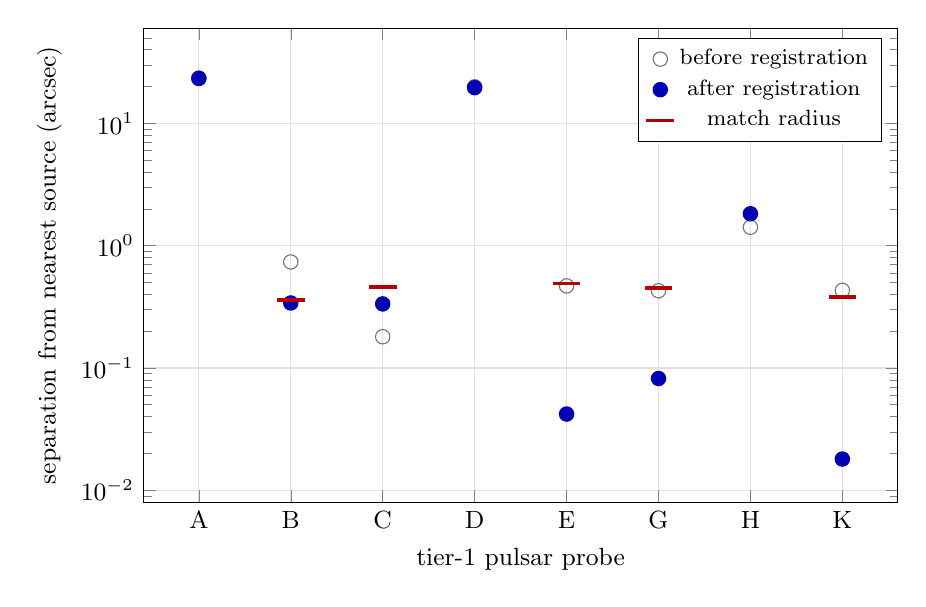
\begin{tikzpicture}
\begin{semilogyaxis}[
  width=0.92\linewidth, height=7.6cm,
  xlabel={tier-1 pulsar probe}, ylabel={separation from nearest source (arcsec)},
  xtick={1,2,3,4,5,6,7,8},
  xticklabels={A,B,C,D,E,G,H,K},
  xmin=0.4, xmax=8.6, ymin=0.008, ymax=60,
  legend style={font=\footnotesize, at={(0.98,0.98)}, anchor=north east},
  grid=major, grid style={black!12},
  tick label style={font=\small}, label style={font=\small},
]
\addplot[only marks, mark=o, mark size=2.6pt, black!55] coordinates {(1,23.468) (2,0.736) (3,0.180) (4,19.915) (5,0.469) (6,0.428) (7,1.415) (8,0.431)};
\addlegendentry{before registration}
\addplot[only marks, mark=*, mark size=2.6pt, blue!70!black] coordinates {(1,23.316) (2,0.340) (3,0.334) (4,19.596) (5,0.042) (6,0.082) (7,1.825) (8,0.018)};
\addlegendentry{after registration}
\addplot[only marks, mark=-, mark size=5pt, red!70!black, very thick] coordinates {(2,0.36) (3,0.46) (5,0.49) (6,0.45) (8,0.38)};
\addlegendentry{match radius}
\end{semilogyaxis}
\end{tikzpicture}
\caption{Tier-1 separations before and after the $(-0.072\as, +0.422\as)$ frame registration, with the match radius of each registered association marked. Registration moves B and K below their radii, tightens E and G inside radii they already satisfied, and moves H further away. A and D have no catalogue source within $19\as$ under either frame. Values from \texttt{analysis/results\_omega\_cen\_5anchor.json}.}
\label{fig:separations}
\end{figure}

\subsection{The MSP H association is discrepant}
\label{sec:results-h}

\citet{ZhaoHeinke2023} quote an offset of $0.73\as$ between MSP~H and their X-ray source h1, and cross-reference h1 to \citet{Henleywillis2018} source 14c. The timing position of \citet{ColomiBernadich2026} sits $1.415\as$ from the catalogue position of 14c, and $1.825\as$ from it after frame registration. The deviation runs in the opposite declination sense to the five anchors, $-1.398\as$ against a $+0.42\as$ median.

\citet{ZhaoHeinke2023} list two X-ray candidates near H, h1 and h2, $1.9\as$ apart, and cross-reference both to 14c. They fit h1 with a power law and assign it to H; they fit h2 with thermal plasma and rule it out as an MSP. After shifting their positions onto the \citet{Henleywillis2018} frame by the mean offset of six common sources ($-0.147 \pm 0.049\as$ in right ascension, $+0.685\as$ in declination; \texttt{analysis/REPORT\_D242.md}), 14c lies $0.08\as$ from h2 and $1.86\as$ from h1, and the registered timing position of \citet{ColomiBernadich2026} lies $0.21\as$ from h1 and $1.83\as$ from 14c. With the declination term alone, as in earlier versions, the separation from h1 is $0.07\as$; both values are an order of magnitude below the distance to 14c. Their quoted positional uncertainties are 95\% radii of $0.40\as$ (h1) and $0.22\as$ (h2). We therefore identify 14c with h2. H is consistent with h1, which has no separate entry in the 233-source catalogue, and we drop H from the registration anchors. The flux of h1, about three times the quoted core limit, and the soft colour of 14c leave open whether h1 went undetected or contributes a minor share of 14c; an inspection of the 222\,ks image at the h1 position would settle it.

The consequence for this paper is bounded. Including H as a sixth anchor moves both medians by $\leq0.011\as$ and changes no match status in Table~\ref{tab:tier1}. The finding matters as a data-quality result about the 14c cross-reference.

\subsection{Classification census}
\label{sec:results-class}

Published classes are taken verbatim from \citet{Henleywillis2018} and are not re-derived; the parenthesis convention of that catalogue marks non-members. The parse reproduces the paper's own abstract composition (Table~\ref{tab:classes}): 18 cataclysmic variables and candidates, one quiescent low-mass X-ray binary, four member variable stars, five anomalous-RGB or sub-subgiant stars, and one CH star, against 45 identifications in total.

\begin{table}[tbp]
\centering
\small
\caption{Published class census over all 233 catalogue sources \citep{Henleywillis2018}, membership as published. Source 24f is counted here under its published class (Section~\ref{sec:data-24f}).}
\label{tab:classes}
\begin{tabular}{llc}
\toprule
Class & Published membership & $n$ \\
\midrule
unidentified & no published statement & 188 \\
CV / CV candidate & member & 18 \\
AGN / AGN candidate & non-member & 9 \\
anomalous RGB / sub-subgiant & member & 5 \\
variable star & member & 4 \\
variable star & non-member & 4 \\
foreground star & non-member & 3 \\
quiescent LMXB & member & 1 \\
CH star (symbiotic candidate) & member & 1 \\
\bottomrule
\end{tabular}
\end{table}

Membership probabilities under the external normalisations of Section~\ref{sec:method-membership} are given in Table~\ref{tab:membership} and plotted in Figure~\ref{fig:membership}. The spread across assumptions is the result. Summed membership over the aperture runs from 51.0 to 86.0 sources as the assumed member count moves from 40 to 80 and the flux limit moves between its two settings, and the number of individual sources crossing $P_{\mathrm{member}} > 0.5$ runs from 0 to 67 over the same range. A binary membership label extracted from any single row of that table would be an artifact of the normalisation chosen.

\begin{table}[tbp]
\centering
\small
\caption{Membership sensitivity. Rows are the six combinations of assumed cluster-member count and background flux limit. Sums run over all 233 catalogue sources, not only the 200 inside the $480\as$ aperture; restricted to the aperture, the 60-member, fifth-percentile total would be 68.9 rather than 72.7.}
\label{tab:membership}
\begin{tabular}{llccc}
\toprule
Assumed members & Flux limit & $N(P_{\mathrm{member}}>0.5)$ & $\sum P_{\mathrm{member}}$ & $\sum P_{\mathrm{member}}$ (unidentified) \\
\midrule
40 & core limiting  & 0  & 51.0 & 39.6 \\
40 & 5th percentile & 6  & 55.9 & 43.3 \\
60 & core limiting  & 23 & 67.1 & 52.1 \\
60 & 5th percentile & 38 & 72.7 & 56.5 \\
80 & core limiting  & 55 & 79.9 & 62.2 \\
80 & 5th percentile & 67 & 86.0 & 67.0 \\
\bottomrule
\end{tabular}
\end{table}

\begin{figure}[tbp]
\centering
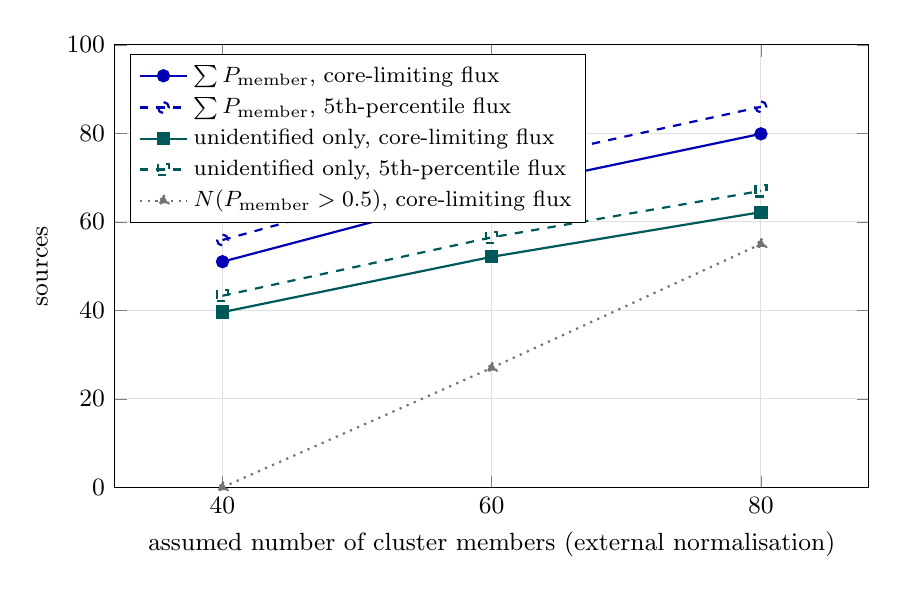
\begin{tikzpicture}
\begin{axis}[
  width=0.92\linewidth, height=7.2cm,
  xlabel={assumed number of cluster members (external normalisation)},
  ylabel={sources},
  xtick={40,60,80}, xmin=32, xmax=88, ymin=0, ymax=100,
  legend style={font=\footnotesize, at={(0.02,0.98)}, anchor=north west, cells={anchor=west}},
  grid=major, grid style={black!12},
  tick label style={font=\small}, label style={font=\small},
]
\addplot[blue!70!black, thick, mark=*] coordinates {(40,51.0) (60,67.1) (80,79.9)};
\addlegendentry{$\sum P_{\mathrm{member}}$, core-limiting flux}
\addplot[blue!70!black, thick, dashed, mark=o] coordinates {(40,55.9) (60,72.7) (80,86.0)};
\addlegendentry{$\sum P_{\mathrm{member}}$, 5th-percentile flux}
\addplot[teal!70!black, thick, mark=square*] coordinates {(40,39.6) (60,52.1) (80,62.2)};
\addlegendentry{unidentified only, core-limiting flux}
\addplot[teal!70!black, thick, dashed, mark=square] coordinates {(40,43.3) (60,56.5) (80,67.0)};
\addlegendentry{unidentified only, 5th-percentile flux}
\addplot[black!55, thick, dotted, mark=triangle*] coordinates {(40,0) (60,27) (80,55)};
\addlegendentry{$N(P_{\mathrm{member}}>0.5)$, core-limiting flux}
\end{axis}
\end{tikzpicture}
\caption{Membership ladder. Summed membership probability over the $480\as$ aperture, and over its unidentified subset, against the assumed external member normalisation at two background flux limits. The count of sources individually exceeding $P_{\mathrm{member}} = 0.5$ (dotted) moves from 0 to 55 over the same range, which is why membership is reported as a summed probability under stated assumptions and not as a label. Values from \texttt{analysis/results\_omega\_cen.json}.}
\label{fig:membership}
\end{figure}

\citet{Platais2024} supply an astrometric census of dark companions in this cluster that the X-ray census here does not capture: from 13 years of HST/WFC3 astrometry of the core, four members carry measured accelerations requiring dark companions of $0.7$--$1.4\,\msun$, at least one of them a neutron-star candidate by their classification. None of the four has a counterpart in the catalogues used here. With the five-anchor frame registration of Section~\ref{sec:results-frame} applied to each position, the nearest catalogue source to any of the four lies $15.4\as$ away, an order of magnitude beyond that source's $95\,\mathrm{per~cent}$ error radius, and the nearest pulsar position lies $32\as$ away; the astrometric and X-ray inventories of the cluster's compact objects are disjoint at this depth.

\subsection{Background accounting}
\label{sec:results-agn}

Table~\ref{tab:agn} gives the expected background over the $0.05585\,\mathrm{deg^{2}}$ aperture at four candidate flux limits. The limit adopted for the residual is the fifth-percentile soft flux of the catalogue itself, $1.4\times10^{-16}\,\mathrm{erg\,cm^{-2}\,s^{-1}}$, giving 146.9 expected background sources with a bracket of 92.4 to 215.5. The core limiting flux, quoted by the source catalogue as $3\times10^{-16}\,\mathrm{erg\,s^{-1}\,cm^{-2}}$ in its own (0.5--6\,keV) band, is converted to the soft (0.5--2\,keV) band by a factor of $0.377$ before it is looked up on the soft-band $\log N$--$\log S$ relation; that factor assumes the same $\Gamma=1.4$ unabsorbed power-law spectrum the catalogue itself uses for all its flux columns (Section~\ref{sec:data-xray}), giving $1.13\times10^{-16}\,\mathrm{erg\,s^{-1}\,cm^{-2}}$ and 167.0 expected sources, 14 per cent above the adopted limit's 146.9, with the two limits' brackets (104.5 to 246.7 and 92.4 to 215.5) overlapping over most of their range. The faintest tabulated flux lies below the fitted range of the \citet{Moretti2003} relation and is shown only to mark where extrapolation begins.

\begin{table}[tbp]
\centering
\small
\caption{Expected extragalactic background over the $480\as$ aperture at four candidate flux limits, from \citet{Moretti2003}. Brackets from the published parameter uncertainties used as symmetric widths. The row marked $\dagger$ lies below the relation's fitted flux range.}
\label{tab:agn}
\begin{tabular}{lcccc}
\toprule
Flux limit & $S$ ($\mathrm{erg\,cm^{-2}\,s^{-1}}$) & $N$ per $\mathrm{deg^{2}}$ & Expected in field & Bracket \\
\midrule
core limiting, scaled to soft & $1.13\times10^{-16}$ & 2991  & 167.0 & 104.5--246.7 \\
faintest tabulated soft$^{\dagger}$ & $1.00\times10^{-17}$ & 12852 & 717.8 & 417.2--1140.5 \\
fifth percentile soft (adopted) & $1.40\times10^{-16}$ & 2630  & 146.9 & 92.4--215.5 \\
median soft & $9.90\times10^{-16}$ & 787   & 43.9  & 29.4--60.7 \\
\bottomrule
\end{tabular}
\end{table}

The background comparison of Figure~\ref{fig:lognlogs} has essentially no power to register an excess at this depth, and that limitation is structural rather than a property of these particular data. The bracket at the adopted limit is $92.4$--$215.5$, a half-width of $\sim$61, itself close to five times the Poisson $\sqrt{145}\simeq12$; over the sampled grid, 81 of 90 points fall inside the bracket and the nine that do not exceed it by at most $2.1$ against a Poisson error of $7.5$ there. No attainable source count at this depth can jointly clear the bracket's edge and the Poisson noise on top of it, so the $\log N$--$\log S$ panel is best read as scale-setting, fixing the background against which the colour-flux region and target list are built, rather than as a test capable of detecting a cluster excess. The inferential weight of this paper rests on the colour-flux region (Section~\ref{sec:results-msplike}) and the follow-up list (Section~\ref{sec:targets}), not on this panel.

\subsection{The residual census}
\label{sec:results-residual}

Inside the $480\as$ aperture the catalogue holds 200 sources, of which 41 carry a published identification (27 published members, 14 published non-members) and 159 do not. Seven of the aperture's 200 sources carry a Henleywillis identifier cross-referenced to an MSP X-ray counterpart; one of those, 14c, is the h2 identification of Section~\ref{sec:results-h} and is not counted as a confirmed counterpart, and another, source 24f, is already published under an optical class (Section~\ref{sec:data-24f}) and so sits in the identified 41, not the unidentified 159, leaving five confirmed counterparts inside the unidentified population: 13d, 23g, 11f, 21d and 32d. The like-for-like residual, matching observed to expected at the same adopted flux limit, is
\begin{equation}
N_{\mathrm{residual}} = 145 - 146.9\,(92.4\text{--}215.5) = -1.9\ (-70.5,\ +52.6),
\label{eq:residual}
\end{equation}
where 145 is the count of unidentified sources carrying a tabulated soft flux at or above the adopted limit exactly. On the sampled log-flux grid nearest that limit ($1.3731\times10^{-16}$), the discretised curve of Figure~\ref{fig:lognlogs} reads $145 - 148.6 = -3.6$; the two differ only by grid discretisation and both are negative. A third quantity, 159 minus 146.9 $= 12.1$, subtracts the same background from the full unidentified population rather than from the at-limit population it was fitted to, a comparison of mismatched limits; it is not the headline of this paper and is retained here only because it is the quantity earlier drafts printed (Appendix~\ref{app:revisions}).

Three counts run through this accounting and are not interchangeable: 159, every unidentified source inside the aperture; 145, those of the 159 carrying a tabulated soft flux at or above the adopted limit, which Equation~\eqref{eq:residual} uses; and 147, an erroneous intermediate that arises from mislabelling two hard-only sources (22g, 43i, each with zero tabulated soft flux and a non-zero medium/total flux) as being at or above the limit when they are in fact below it, a code-level truthiness bug (\texttt{if flux\_soft} misreads \texttt{0.0} as ``no value'' rather than ``below limit''; the fix is \texttt{is not None}). 147 does not appear in any number this paper reports and is documented here only to close the count.

The residual is background-dominated. Its central value is 1.3\,per~cent of the quantity subtracted and its bracket spans zero by a wide margin on both sides. The conservative reading is that the unidentified population inside this aperture, matched at the adopted flux limit, is consistent with the extragalactic background alone, and that no excess is required by these data at this flux limit. Nothing in the rest of this paper should be read as claiming otherwise. What the residual does supply is a scale: an identification programme working through this field is working against a background that supplies of order 150 sources, and any cluster population it hopes to extract is a minority of the unidentified list.

\begin{figure}[tbp]
\centering
\includegraphics[width=0.92\linewidth]{../figs/fG_expand_lognlogs.png}
\caption{The residual, drawn rather than quoted. Top: cumulative count of
unidentified sources inside the $480\as$ aperture above a soft-band flux limit,
against the \citet{Moretti2003} background expectation over the same solid angle
with its published parameter uncertainties propagated as a bracket. Bottom: the
same difference on a linear scale. The observed curve stays inside the bracket at
90\,per~cent of the sampled limits; where it crosses the upper edge, between
$4$ and $13\times10^{-16}\,\mathrm{erg\,cm^{-2}\,s^{-1}}$, it does so by at most
2.1 sources against a Poisson error of 7.5 on the count there, so the crossing
carries no excess. The faint-end flattening of the observed curve is catalogue
incompleteness. The drawn curve carries the 145 unidentified sources with a
tabulated soft flux at or above the adopted limit; Equation~\eqref{eq:residual}
matches them against the background expectation at that same limit, out of the
159 unidentified sources in the aperture overall.
Values from \texttt{../figs/fG\_expand\_lognlogs.json}.}
\label{fig:lognlogs}
\end{figure}

Figure~\ref{fig:lognlogs} draws the same accounting continuously in flux. What the
bracket does to the residual is visible directly: it is wider than the residual at
every limit sampled, and at the adopted limit the observed curve and the background
expectation cross almost exactly. Two of the 159 unidentified sources (22g, 43i)
carry a tabulated hard flux but a zero tabulated soft flux and so drop below the
soft-flux limit rather than sitting above it; they are correctly excluded from the
145-source drawn curve, and the 147 figure quoted in earlier versions (Appendix~\ref{app:revisions})
came from misreading their zero soft flux as ``no value'' rather than ``below
limit'' (see the note after Equation~\eqref{eq:residual}).

Three accounting conventions change the number and are stated here. Published non-member AGN identifications sit in the identified column, so the subtraction removes a predicted background from a population that already excludes background sources someone has taken the trouble to identify, which biases the residual low. The aperture excludes 33 catalogue sources from both sides, so this is not a statement about the full 233. And the five in-aperture unidentified MSP X-ray counterparts are retained in the unidentified column, since the catalogue's own optical-identification field predates the pulsar timing set; removing them would lower the residual by that count, well inside the quoted bracket. Under the membership model of Table~\ref{tab:membership} (60 assumed members, fifth-percentile limit) the 145 sources of Equation~\eqref{eq:residual} carry 47.6 expected members, because that model spreads the background over all 200 aperture sources while Equation~\eqref{eq:residual} charges all of it to these 145; the 47.6 follows from the assumed member count and lies inside the residual's bracket, below its upper edge of $+52.6$.

\subsection{The MSP-like region}
\label{sec:results-msplike}

The confirmed counterparts define a region in the colour-flux plane from this cluster's own data. Four of them ($n=4$: 23g, 11f, 24f, 21d) carry both a tabulated colour and a flux and anchor it; a fifth recovered counterpart lacks a tabulated colour and is dropped. The flux axis of both region constructions is the catalogue's total (0.5--6\,keV) band flux, $F_{X,\mathrm{tot}}$, not the soft (0.5--2\,keV) flux $F_{\mathrm{soft}}$ printed in Tables~\ref{tab:targets} and \ref{tab:twelve}; the two bands are not interchangeable (Section~\ref{sec:data-xray}), and a reader working from either table's printed flux column alone cannot reproduce the region boundary. The primary construction is a bounding box on those same four anchors, with edges $\log F_{X,\mathrm{tot}} \in [0.80, 1.56]$ ($6.3$--$36.4\times10^{-19}\,\mathrm{W\,m^{-2}}$) and colour $\log(\mathrm{soft}/\mathrm{hard}) \in [-0.20, +0.68]$: counting unidentified sources inside it gives 39, of which 14.85 survive membership weighting at the adopted normalisation. A four-anchor ellipse on the same $n=4$ anchors, reported as a secondary and wider construction, gives 53 (19.44 weighted). Both counts rest entirely on the four anchors, and the leave-one-out recounts say so: dropping any one anchor moves the box count over 15--39 and the ellipse count over 7--74 (membership-weighted 6.5--14.9 and 2.0--14.9), because each anchor sets an edge of one construction or the other. The upper-bound reading is unaffected (every recount is still an upper bound), but the point values 39 and 53 should be quoted with these ranges attached. Numbers in \texttt{paper/g/calc7/g\_calc7\_anchor\_loo.json}. Eleven unidentified sources carry neither a colour nor a flux and cannot be placed in the plane at all. Neither region screens for background AGN, so the 39 and 53 counts are upper bounds on MSP-like membership rather than membership estimates.

\begin{figure}[tbp]
\centering
\includegraphics[width=0.92\linewidth]{../figs/fG_expand_colourflux.png}
\caption{The colour-flux plane inside the $480\as$ aperture, flux axis
$\log F_{X,\mathrm{tot}}$ (total, 0.5--6\,keV band; not the soft-band
$F_{\mathrm{soft}}$ of Tables~\ref{tab:targets}/\ref{tab:twelve}), with the primary
bounding box and the secondary four-anchor ellipse drawn on the four confirmed
counterparts that anchor them. Both regions are constructed from the four stars
plotted inside them, so the anchors' position in the region is a construction and
not a test of it. The box holds 39 unidentified sources and the ellipse 53, and
neither screens for background AGN, which is why both counts are upper bounds.
Twelve aperture sources lack a colour or a flux and do not appear.
Values from \texttt{../figs/fG\_expand\_colourflux.json}.}
\label{fig:colourflux}
\end{figure}

This is not the ``more than 30 MSP-like'' count of \citet{Henleywillis2018}. That criterion compares against MSPs in other clusters and is not tabulated in the source paper, so it cannot be reproduced from the machine-readable table. The region used here is defined from four counterparts in this cluster, a different construction with a different systematic. The two numbers are not interchangeable, and the numerical proximity of 39 to ``more than 30'' is a coincidence of construction rather than a confirmation.

\section{The population disagreement}
\label{sec:tension}

Two published estimates of the total pulsar population of \ocen{} are available and they disagree by a factor of 54 (324 against 6). \citet{Yin2024} report an empirical-Bayesian escape-velocity scaling relation that predicts 324 pulsars at this cluster's escape velocity of $62.2\,\mathrm{km\,s^{-1}}$ (the \citealt{Yin2024} scaling-relation convention; Paper H's fast-star selection threshold uses a different escape-velocity convention, $62.8\,\mathrm{km\,s^{-1}}$ from the Baumgardt \& Hilker (2018) catalogued central dispersion, distance-scaled; the two differ by $\sim$1\,per~cent and are not the same quantity). The encounter-rate estimate they tabulate alongside it gives 6.

Against 19 known pulsars those totals imply 305 and $-13$ undiscovered, the second truncated at zero. The X-ray detection fraction measured in this cluster depends on which denominator is used: \citet{ZhaoHeinke2023} found 11 counterparts among the 18 MSPs known and searched at the time of their work (0.611), while 19 pulsars are known today and the 19th was never searched, not a non-detection, so the conservative variant against today's full count is 11 of 19 (0.579). We carry both rather than choosing: applying 0.611 gives 186.4 and applying 0.579 gives 176.6 X-ray-detectable undiscovered pulsars from the escape-velocity model; the encounter-rate model gives 0.0 under either fraction, because its total of 6 lies below the 19 pulsars already known and the undiscovered count is truncated at zero (Table~\ref{tab:pop}).

\begin{table}[tbp]
\centering
\small
\caption{Population predictions from \citet{Yin2024}, carried as a bracket. The final two columns apply the X-ray detection fraction measured in this cluster under its two denominators: 0.611 (11 of the 18 MSPs \citet{ZhaoHeinke2023} searched) and 0.579 (11 of the 19 known today, conservative). The encounter-rate undiscovered count is $6-19=-13$, truncated at zero.}
\label{tab:pop}
\begin{tabular}{lcccc}
\toprule
Model & Predicted total & Undiscovered & X-ray-detectable (0.611) & X-ray-detectable (0.579) \\
\midrule
escape velocity & 324 & 305 & 186.4 & 176.6 \\
encounter rate  & 6   & 0   & 0.0   & 0.0 \\
\bottomrule
\end{tabular}
\end{table}

The X-ray-detectable escape-velocity number, 186.4 (176.6 at the all-19 fraction), exceeds the magnitude of the matched-limit residual, 1.9, by a factor of about 98 (93), exceeds the mismatched-limit 12.1 by more than one order of magnitude, and exceeds the full unidentified count of 159 once the background is not subtracted. That bounds the extrapolation, the assumed detection fraction, or the background subtraction, and this analysis does not decide which. Three reasons keep each candidate live.

\textbf{The extrapolation.} The \citet{Yin2024} relation was fitted on FAST-visible clusters. \ocen{} at $\delta = -47^{\circ}$ is not FAST-visible, so applying the relation here reaches outside the sample it was fitted on, in a cluster whose escape velocity places it at the top of the predicted range.

\textbf{The detection fraction.} The measured 0.611 (or 0.579 against today's full known count) is the fraction of searched pulsars with a Chandra counterpart. Applying it to the undiscovered population assumes those pulsars share the X-ray luminosity distribution of the discovered ones. Radio-faint or large-radius pulsars need not, and the discovered set is selected in ways that correlate with X-ray brightness, so either fraction is more plausibly an upper bound than an unbiased estimate.

\textbf{The background subtraction.} Eddington bias inflates the faint fluxes on which the background limit is computed, which makes the expected background a lower bound and the residual an upper bound. Correcting the residual downward would widen the gap rather than close it.

Adjudicating it requires the identification work this census is meant to enable, not a preference asserted here.

\section{A ranked candidate list}
\label{sec:targets}

The stated purpose of a census of this kind is to supply a target list, so this
section supplies one. Table~\ref{tab:targets} ranks the 39 unidentified sources
inside the primary colour-flux region for follow-up. The full ranked pool, with
positions, all three chance-coincidence estimators and every flag, ships as
\texttt{../figs/fG\_target\_list.json}.

\subsection{Pre-registration of the ranking rule}
\label{sec:targets-rule}

The rule was written down and committed to the project record before any candidate
score existed, as Section~1 of the work-unit editlog
(\texttt{board/notes/G-EXPAND-1-EDITLOG.md}). It scores each candidate

\begin{equation}
R = P_{\mathrm{member}} \times \left(1 - \pchance{}\right),
\end{equation}

with $P_{\mathrm{member}}$ the spatial membership probability of
Section~\ref{sec:method-membership} under the adopted normalisation
($N_{\mathrm{mem}} = 60$, background at the fifth-percentile soft limit), and
\pchance{} the largest of the three estimators of Section~\ref{sec:method-chance}
evaluated with the candidate treated as its own probe and removed from the
comparison catalogue. Ties break by soft flux. No threshold is applied to either
factor: the whole pool is ranked and the first twenty are printed. The adoption is
not load-bearing for the ranking: re-scoring the pool under all six rows of
Table~\ref{tab:membership} changes no position in the top twenty (Spearman
$\rho = 1.00$ in every row), because the score ordering is a cluster-centric-radius
ordering under any of them (\texttt{paper/g/calc7/g\_calc7\_anchor\_loo.json}). This
invariance is an analytic property of the ranking rule, not an empirical robustness
result: $P_{\mathrm{member}}$ is strictly decreasing in cluster-centric radius under
every normalisation in Table~\ref{tab:membership}, $(1-\pchance{})$ moves no
candidate by more than one place (below), and their product therefore reduces to a
radius ordering under any of the six rows by construction. No re-scoring could have
produced a different ranking, so the invariance tests the rule's algebra rather than
the data.

The reason for fixing the rule in advance shows up in what the list then looks
like.

\textbf{The chance factor barely moves the ranking.} Over the whole pool the three estimators
return between $1.8\times10^{-4}$ and $3.2\times10^{-3}$, so $(1-\pchance{})$ never
moves a candidate more than one place. The ordering is the membership probability,
which under a spatial model is a monotonic function of cluster-centric radius. The
rank column is therefore close to a radius ordering, and a reader should treat it
as one. That is a property of the data rather than of the rule: with a catalogue
this shallow and error circles this small, positional confusion is not what limits
follow-up in this cluster.

\textbf{Four rows are already identified.} The pool is defined by the absence of a
published optical identification, which is the catalogue's own field. Seven of the
19 pulsars carry a cross-reference to a Henleywillis identifier (Section~\ref{sec:data-counterparts}), but one of those seven, 24f, is already published under an
optical class (Section~\ref{sec:data-24f}) and so is not in the unidentified pool
at all; the six that are unidentified in this catalogue's own field carry no
optical identification. Four
of them survive the colour and flux cuts and rank in the top twenty (11f, 21d, 23g
and 32d, flagged \texttt{c}). Three of those four are also the anchors that define
the box, so their high rank is circular twice over and is not evidence that the
score works. A follow-up programme would drop all four; the pre-registered pool
retains them, and Table~\ref{tab:targets} flags rather than removes them. With them
removed the first five entries are 12c, 11e, 13g, 22l and 24j.

\textbf{No row is an identification.} Section~\ref{sec:results-msplike}'s
upper-bound caveat applies unchanged: the region carries no AGN screen, and at the
adopted limit the background expectation over this aperture is 146.9 sources. Most
of this list is expected to be background, and the ordering is of follow-up effort
rather than of likelihood.

\begin{table}[tbp]
\centering
\small
\caption{Top twenty of the 39-source candidate pool under the pre-registered rule
of Section~\ref{sec:targets-rule}. Radius is cluster-centric; colour is
$\log(\mathrm{soft}/\mathrm{hard})$; $F_{\mathrm{soft}}$ (soft, 0.5--2\,keV) and
$F_{X,\mathrm{tot}}$ (total, 0.5--6\,keV) are both in
$10^{-16}\,\mathrm{erg\,cm^{-2}\,s^{-1}}$; the colour-flux region of
Section~\ref{sec:results-msplike} and Figure~\ref{fig:colourflux} is built on
$F_{X,\mathrm{tot}}$, not $F_{\mathrm{soft}}$. Flags: \texttt{a} box anchor,
\texttt{c} confirmed MSP X-ray counterpart, \texttt{n} source new in the 2012 data,
\texttt{v} tabulated 2012/2000 flux ratio beyond a factor of two, \texttt{l} fewer
than ten corrected medium-band counts, \texttt{e} inside the box but outside the
four-anchor ellipse. Chance values are rounded half up. Positions and the remaining nineteen rows are in
\texttt{../figs/fG\_target\_list.json}; $F_{X,\mathrm{tot}}$ from
\texttt{data/xray\_census.json}.}
\label{tab:targets}
\begin{tabular}{rlrrrrrrrl}
\toprule
Rank & Source & $r$ (\as) & colour & $F_{\mathrm{soft}}$ & $F_{X,\mathrm{tot}}$ & $P_{\mathrm{member}}$ & $10^{3}\pchance{}$ & $R$ & flags \\
\midrule
1 & 12c & 36 & $+0.22$ & 4.0 & 8.6 & 0.612 & 0.5 & 0.612 & n \\
2 & 11e & 50 & $+0.00$ & 3.6 & 9.1 & 0.601 & 0.4 & 0.601 & n \\
3 & 13g & 70 & $+0.12$ & 4.8 & 9.1 & 0.580 & 0.5 & 0.580 & n \\
4 & 22l & 79 & $+0.14$ & 6.2 & 11.6 & 0.569 & 0.5 & 0.568 & n \\
5 & 11f & 95 & $+0.17$ & 4.1 & 6.3 & 0.547 & 0.6 & 0.547 & acn \\
6 & 24j & 105 & $+0.50$ & 7.4 & 11.3 & 0.532 & 0.6 & 0.531 & n \\
7 & 21d & 113 & $-0.20$ & 16.0 & 36.4 & 0.520 & 0.8 & 0.520 & ac \\
8 & 21e & 116 & $+0.63$ & 13.9 & 22.6 & 0.515 & 1.3 & 0.515 & e \\
9 & 23g & 118 & $+0.68$ & 5.5 & 9.2 & 0.513 & 0.7 & 0.512 & acn \\
10 & 24d & 129 & $+0.37$ & 6.4 & 11.9 & 0.496 & 0.5 & 0.495 & -- \\
11 & 23e & 132 & $+0.29$ & 3.3 & 6.5 & 0.491 & 1.3 & 0.490 & ln \\
12 & 21f & 132 & $+0.64$ & 6.9 & 11.3 & 0.491 & 1.6 & 0.490 & n \\
13 & 24b & 136 & $+0.38$ & 6.0 & 10.9 & 0.483 & 0.6 & 0.483 & -- \\
14 & 22d & 140 & $+0.34$ & 7.3 & 12.2 & 0.478 & 1.5 & 0.478 & v \\
15 & 34e & 150 & $+0.09$ & 6.0 & 11.3 & 0.461 & 0.5 & 0.461 & n \\
16 & 34h & 167 & $+0.06$ & 4.5 & 9.6 & 0.434 & 0.4 & 0.434 & n \\
17 & 31c & 180 & $+0.40$ & 6.9 & 9.8 & 0.414 & 0.8 & 0.414 & v \\
18 & 31g & 181 & $+0.15$ & 5.0 & 8.9 & 0.412 & 0.7 & 0.412 & n \\
19 & 32d & 195 & $+0.44$ & 5.4 & 10.1 & 0.391 & 2.8 & 0.390 & c \\
20 & 31e & 195 & $+0.15$ & 3.3 & 7.1 & 0.391 & 3.2 & 0.390 & n \\
\bottomrule
\end{tabular}
\end{table}

\section{Discussion}
\label{sec:discussion}

\subsection{What would identify the residual}
\label{sec:disc-future}

The residual is an input to identification work, and the useful output of this paper is a specific list of what that work requires. Each item below is a concrete, currently blocked step, ordered by cost.

\textbf{The missing pulsar positions.} F, J, M, O, P and R carry no position in \citet{ColomiBernadich2026}. \citet{Chen2023} print one for each, but five of the six (F, M, O, P, R) are beam centres at about $\pm1$\,s in right ascension and $\pm6\as$ in declination, unusable against the tier-1 radii. Pulsar J ($\pm1\as$ per axis) is the one recoverable probe, and it is run here as the sixth tier-2 probe: it lies $11.0\as$ from source 22c and does not match (Section~\ref{sec:results-match}).

\textbf{The counterpart-chain check.} The H--14c cross-reference of Section~\ref{sec:results-h} rests on 14c being h2. The remaining routes are new Chandra astrometry of the h1/h2 pair or a blend check of 14c in the \citet{Henleywillis2018} data, and both need data beyond the published tables.

\textbf{Exposure-map membership.} The degeneracy of Section~\ref{sec:method-membership} is instrumental and is fixed by the Chandra exposure map, which turns a spatial fit that cannot separate the cluster profile from the sensitivity profile into one that can. Membership would then be fitted rather than normalised externally, and the six-row sensitivity table of Table~\ref{tab:membership} would collapse to one row with an error bar.

\textbf{Variability with epoch-resolved data.} No variability analysis appears in this paper. Both the 2000 and 2012 Chandra epochs exist and \citet{Henleywillis2018} tabulate a flux ratio between them, but the Chandra Source Catalog (releases 2.1 and 2.2) carries only the two 2012 observations (ObsIDs 13726, 13727; 3.1\,d baseline) for these sources, so catalogue-level epoch data reach no further back than 2012, and a single published ratio does not support a statistically valid variability test at these count rates. This is the clearest gap between what this paper does and what a full identification programme needs, since variability is what separates quiescent binaries from background AGN when colour does not.

\textbf{Deeper radio positions.} Sub-arcsecond positions for the tier-2 pulsars would move six probes out of a tier whose uncertainty rule is a convention of ours rather than a measurement.

\subsection{The census as an anomaly screen}
\label{sec:disc-anomaly}

A complete accounting of a cluster's X-ray sources doubles as a screen for sources fitting no known class, a standard byproduct of catalogue work worth one sentence of acknowledgement in a series that elsewhere considers non-astrophysical hypotheses \citep{Swanson2026Engineered}. This census does not perform that screen. The residual computed here is background-dominated, consistent with zero, and defined by the absence of an optical identification rather than by any positive property; treating it as a population of anomalies would require the identification work Section~\ref{sec:disc-future} lists as outstanding, and until that work is done the residual carries no information about the nature of its members.

\section{Conclusion}
\label{sec:conclusion}

We have cross-matched the 233-source Chandra catalogue of \citet{Henleywillis2018} against the 19-pulsar timing set of \citet{ColomiBernadich2026}, validated the pipeline on 47~Tucanae first, and reported what is left.

The control recovers 18 of 21 known counterparts at the 95\,per~cent match radius and misses the three rows the control catalogue itself flags. The \ocen{} Chandra frame carries a measured $+0.42\as$ declination offset against the radio frame; registering it takes tier-1 matches from three of eight to five of eight, and the five registered associations sit between $0.02\as$ and $0.34\as$ with chance-coincidence probabilities below $2.3\times10^{-3}$ under three independent estimators. MSP~H's timing position is consistent with the X-ray source h1 ($0.21\as$) and lies $1.83\as$ from 14c, which matches h2; H is not used as an anchor (Section~\ref{sec:results-h}).

The residual census inside a $480\as$ aperture, matched at the same flux limit, is $-1.9$ unidentified sources $(-70.5, +52.6)$ against a background expectation of 146.9 (92.4--215.5), which is to say it is consistent with the background alone. 39 (primary box) or 53 (secondary ellipse) unidentified sources fall in a colour-flux region defined by this cluster's own confirmed counterparts, two constructions built differently from the catalogue's own ``more than 30'' and not interchangeable with it or with each other. The two published population predictions differ by a factor of 54, and the X-ray-detectable part of the larger, 186.4 (176.6), exceeds the magnitude of the residual by a factor of about 98 (93), which bounds the extrapolation, the detection fraction, or the background subtraction without deciding among them. The practical output is Table~\ref{tab:targets}, a ranked follow-up list under a rule fixed before the ranking was computed, together with the epoch-comparison depth each entry would require.

\section*{Data availability}

The analysis pipeline (\texttt{crossmatch.py}, \texttt{classify.py}, \texttt{residual.py}, \texttt{run\_g.py}), its fixed seed, its two results files and the mechanical analysis report accompany this paper under \texttt{paper/g/analysis/}. The vendored source catalogues, their checksums and their provenance record are under \texttt{paper/g/data/}. Both source catalogues are public at VizieR (\texttt{J/MNRAS/479/2834} and \texttt{J/MNRAS/472/3706}). The v1.2 figures, the ranked candidate list and the epoch-comparison table are produced by \texttt{paper/figs/fG\_expand\_v1.py}, which reproduces and asserts the analysis of record before computing anything new; the candidate list is machine-readable at \texttt{../figs/fG\_target\_list.json}.

\appendix

\section{Caveat checklist}
\label{app:caveats}

The following are stated as limitations of this analysis and are not corrected for.

\begin{enumerate}
\item \textbf{Eddington bias.} Fluxes near the detection limit are biased high, so a background count computed above a limit derived from those same fluxes is a lower bound on contamination. No deboosting is possible without the detection-significance distribution, which the vendored table does not carry.
\item \textbf{Completeness varies with off-axis angle} across the ACIS-I field. A single flux limit is applied over the whole area, which overestimates the effective depth at large radius and therefore overestimates the background count there while underestimating the true source count. This pushes the residual in the opposite direction from Eddington bias above: Eddington bias makes the background estimate too low (residual biased up), radial incompleteness makes it too high at large radius (residual biased down). Neither correction is quantified here, both are invoked only qualitatively, and their combined scale relative to the $-1.9$ (92.4--215.5-bracket) residual is unmeasured; a reader should treat the residual's true systematic uncertainty as wider than the quoted statistical bracket alone.
\item \textbf{No variability analysis} is performed. Catalogue epoch data cover only the 3.1\,d 2012 baseline; the 2000 epoch would need reprocessing of the 2000 event data. The single tabulated 2012/2000 flux ratio does not support a test with Poisson-limited errors. Explicitly out of scope, and the largest departure from what a full identification programme requires. Appendix~\ref{app:variability} states what the missing work would cost without doing it.
\item \textbf{The residual is an input to future identification work.} It is not a detection and it is not evidence for any hypothesis.
\item \textbf{Chance-coincidence rates} are reported per probe by three independent estimators and are never collapsed into one number.
\item \textbf{Membership} is reported as a probability under stated external normalisations, never as a binary label, and every published membership statement is carried alongside rather than overwritten.
\item \textbf{The tier-2 positional uncertainty rule} is a convention of this analysis (one unit in the last quoted digit), not a value stated by the source paper.
\item \textbf{The escape-velocity population relation} was fitted on FAST-visible clusters and \ocen{} is not FAST-visible, so its prediction here is an extrapolation.
\item \textbf{The background-relation parameter uncertainties} are published asymmetrically and are applied here as symmetric steps in the two parameters; the resulting bracket in $N$ ($92.4$--$215.5$ about $146.9$) is asymmetric and is carried as computed.
\item \textbf{The internal membership fit is degenerate} and is reported as a diagnostic only; membership uses external normalisations throughout.
\item \textbf{The control is an optimistic bound.} The control catalogue was itself astrometrically registered against its MSP truth set, so control recovery bounds match performance from above rather than testing astrometry independently.
\item \textbf{The candidate ranking is a follow-up ordering}, not a set of identifications. Its rule was fixed before it was computed, its chance-coincidence factor is numerically inert, and four of its top twenty rows are already-identified MSP counterparts that the pre-registered pool definition retains.
\item \textbf{The epoch-comparison table of Appendix~\ref{app:variability}} assumes the shallower epoch differs from the deeper one only in exposure. It does not, so the tabulated sensitivity is a floor.
\item \textbf{Five pulsars are absent} from the cross-match because \citet{ColomiBernadich2026} carry no usable position for them (they have only beam-centre positions in \citet{Chen2023}, too coarse for the tier-1 radii), so every match count is conditional on a 14-probe subset of the 19-pulsar timing set.
\end{enumerate}


\section{Cost of an epoch comparison}
\label{app:variability}

Variability is absent from this paper and Appendix~\ref{app:caveats} lists that
absence as its largest departure from a full identification programme. This
appendix states what that work would cost. It analyses no epoch-resolved data and
classifies
no source as variable; it converts the catalogue's own counts into the sensitivity
a two-epoch comparison would have.

The catalogue's counts come from the 2012 ACIS-I exposure alone, 173.7 and
48.5\,ks \citep{Henleywillis2018}. The other deep Chandra epoch of this field is
the $\sim$70\,ks exposure of \citet{Haggard2009}, so a second epoch collects
$r = 0.315$ of the counts at constant flux. Propagating Poisson errors on the two
rates, the smallest flux ratio a three-sigma comparison could detect is
$R_{\min} = \exp[3(1/n_{2012} + 1/n_{2000})^{1/2}]$. Table~\ref{tab:variability}
counts how many sources clear each threshold. Rows are given twice: once
restricted to sources where the shallower epoch expects at least ten counts, which
is where the Gaussian propagation holds, and once without that restriction. The
restriction bites at 31.7 counts in the deep epoch, where $R_{\min}$ is already
2.97, so requiring validity and requiring a factor of three are nearly the same
cut and neither is presented as the answer alone.

\begin{table}[tbp]
\centering
\small
\caption{Sources whose 2012 counts would support a three-sigma detection of a flux
change by the tabulated factor against the $\sim$70\,ks 2000 epoch. The pool
column counts the 39 candidates of Section~\ref{sec:targets}. Columns 2--3 keep
only rows where the shallower epoch expects at least ten counts; columns 4--5 drop
that restriction and are indicative only: the $R_{\min}$ formula assumes Gaussian
propagation on both epochs, an assumption those rows are outside, and their counts
are not to be read as detection forecasts.
Values from \texttt{../figs/fG\_expand\_variability.json}.}
\label{tab:variability}
\begin{tabular}{lcccc}
\toprule
 & \multicolumn{2}{c}{Gaussian regime} & \multicolumn{2}{c}{no validity cut} \\
\cmidrule(lr){2-3}\cmidrule(lr){4-5}
Flux ratio & aperture (200) & pool (39) & aperture (200) & pool (39) \\
\midrule
1.5 & 18 & 0 & 18 & 0 \\
2.0 & 53 & 0 & 53 & 0 \\
3.0 & 98 & 10 & 98 & 10 \\
5.0 & 98 & 10 & 165 & 35 \\
10.0 & 98 & 10 & 194 & 39 \\
\bottomrule
\end{tabular}
\end{table}

The candidate pool is worse placed than the aperture at large. Ninety-eight of the 200
aperture sources sit in the Gaussian regime and 53 would show a factor-of-two
change, but none of those 53 is in the candidate pool: the MSP-like region selects
faint sources. Ranked by detectable flux-change factor rather than by
Table~\ref{tab:targets}'s follow-up rank, the five best-placed pool members
(21d, 41a, 43a, 84f, 74a) need factors of 2.2 to 2.4; the five top-ranked
entries of Table~\ref{tab:targets} (12c, 11e, 13g, 22l, 11f) need factors of
4.0 to 6.0, since follow-up rank orders by membership probability and chance
rate, not by the counts a variability comparison needs.
Reaching a factor of two on the top of Table~\ref{tab:targets} needs new exposure,
not a re-reduction of the archive. The comparison itself carries costs this
arithmetic does not price. The 2000 exposure reaches a limiting flux of
$\sim$$4.3\times10^{-16}\,\mathrm{erg\,cm^{-2}\,s^{-1}}$ against
$\sim$$3\times10^{-16}$ for the 2012 data, and the two reductions differ in
aperture, off-axis angle and extraction, so $R_{\min}$ is a floor rather than a
forecast.

An all-sky survey does not substitute. Four of the 200 aperture sources reach the
eRASS1 50\,per~cent completeness limit of
$5\times10^{-14}\,\mathrm{erg\,cm^{-2}\,s^{-1}}$ \citep{Merloni2024}, and 106 of
the 200 have a catalogue neighbour inside the $26\as$ half-energy width that
eROSITA averages over its field of view \citep{Predehl2021}. Its depth and its beam
each rule it out for this field independently.


\section{Per-source table for the twelve finding-chart candidates}
\label{app:twelvetable}

The finding chart (Fig.~\ref{fig:findingchart}) numbers the twelve highest-ranked non-counterpart candidates of the 39-source colour--flux pool in pre-registered rank order (Sec.~\ref{sec:targets}; \texttt{../figs/fG\_target\_list.json} ranks 1--4, 6, 8, 10--15 after removing the four confirmed MSP counterparts). Table~\ref{tab:twelve} gives the machine-readable row for each, from the vendored census (\texttt{data/xray\_census.json}, byte-parse of \citet{Henleywillis2018} table1.dat) and the ranked pool (\texttt{../figs/fG\_target\_list.json}), with the epoch depth from \texttt{../figs/fG\_expand\_variability.json}. Off-axis angle is proxied by cluster-centric radius $r$ (the Chandra aimpoint is the cluster centre; $\epsilon_{95}$ grows with off-axis angle and is listed) and by the catalogue $\epsilon_{95}$. Net counts are the exposure- and vignetting-corrected 0.5--4.5\,keV counts; flux is the unabsorbed 0.5--2.0\,keV (soft) flux in $10^{-19}$\,W\,m$^{-2}$ ($10^{-16}$\,erg\,cm$^{-2}$\,s$^{-1}$) under the $\Gamma=1.4$ power-law assumed by the source catalogue. Where the 2012/2000 flux ratio is not tabulated the source is new in the 2012 data set and no ratio is computable at this count rate; the ratio floor for a $3\sigma$ change is in Table~\ref{tab:variability}. Tier is the selection tier: all twelve are ``unidentified, inside the 480\as\ aperture, colour and flux both tabulated, inside the $n=4$ primary box''; flags are from the ranked pool (outside-ellipse, low-counts, variable-candidate).

\begin{table}[htbp]
\centering
\small
\caption{Per-source rows for the twelve finding-chart candidates (Fig.~\ref{fig:findingchart}), in chart order. RA/Dec from \texttt{data/xray\_census.json}; $r$ and $\epsilon_{95}$ in arcseconds; $C_{0.5-4.5}$ corrected medium-band counts; $F_{\rm soft}$ unabsorbed 0.5--2.0\,keV flux in $10^{-19}$\,W\,m$^{-2}$; $F_{X,{\rm tot}}$ total flux $10^{-19}$\,W\,m$^{-2}$; $R=F_{12}/F_{00}$ epoch ratio where tabulated; flags from \texttt{../figs/fG\_target\_list.json}. Data as vendored, no re-derivation.}
\label{tab:twelve}
\footnotesize
\begin{tabular}{cllccrrrrrl}
\toprule
Chart & ID & RA (J2000) & Dec (J2000) & $r$ & $\epsilon_{95}$ & $C_{0.5-4.5}$ & $F_{\rm soft}$ & $F_{X,{\rm tot}}$ & $R$ & Flags \\
 & & & & (\as) & (\as) & (corr) & ($10^{-19}$) & ($10^{-19}$) & $F_{12}/F_{00}$ & \\
\midrule
1 & 12c & 13h26m47.945s & $-47$:28:10.74 & 35.7 & 0.41 & 15.5 & 4.0 & 8.6 & --- & n \\
2 & 11e & 13h26m43.279s & $-47$:28:16.18 & 49.6 & 0.43 & 14.6 & 3.6 & 9.1 & --- & n \\
3 & 13g & 13h26m54.065s & $-47$:28:59.06 & 69.8 & 0.41 & 16.9 & 4.8 & 9.1 & --- & n \\
4 & 22l & 13h26m54.828s & $-47$:28:32.66 & 79.1 & 0.40 & 19.6 & 6.2 & 11.6 & --- & n \\
5 & 24j & 13h26m42.326s & $-47$:30:19.33 & 105.4 & 0.45 & 20.9 & 7.4 & 11.3 & --- & n \\
6 & 21e & 13h26m45.206s & $-47$:26:52.25 & 116.3 & 0.39 & 42.3 & 13.9 & 22.6 & 0.96 & e \\
7 & 24d & 13h26m37.399s & $-47$:30:06.97 & 128.7 & 0.49 & 21.2 & 6.4 & 11.9 & 0.98 & --- \\
8 & 23e & 13h26m58.174s & $-47$:29:57.10 & 131.8 & 0.55 & 9.8 & 3.3 & 6.5 & --- & n,l \\
9 & 21f & 13h26m37.860s & $-47$:27:15.51 & 131.8 & 0.48 & 20.6 & 6.9 & 11.3 & --- & n \\
10 & 24b & 13h26m39.312s & $-47$:30:37.06 & 136.4 & 0.50 & 20.0 & 6.0 & 10.9 & 1.02 & --- \\
11 & 22d & 13h26m58.723s & $-47$:27:28.73 & 139.5 & 0.44 & 21.9 & 7.3 & 12.2 & 0.47 & v \\
12 & 34e & 13h26m43.202s & $-47$:31:10.62 & 150.4 & 0.51 & 21.0 & 6.0 & 11.3 & --- & n \\
\bottomrule
\multicolumn{11}{l}{\footnotesize Chart order is pre-registered rank order after removing confirmed MSP counterparts (see Fig.~\ref{fig:findingchart} caption;} \\
\multicolumn{11}{l}{\footnotesize \phantom{Chart} ranks 1--4,6,8,10--15 in \texttt{../figs/fG\_target\_list.json}). $R$ is the catalogue 2012/2000 flux ratio where} \\
\multicolumn{11}{l}{\footnotesize \phantom{Chart} tabulated; ``---'' denotes a new 2012 source with no computable ratio (cf.\ Table~\ref{tab:variability}). Flags:} \\
\multicolumn{11}{l}{\footnotesize \phantom{Chart} n\,=\,new in 2012, e\,=\,inside box but outside the four-anchor ellipse, l\,=\,$<10$ corrected counts, v\,=\,catalogued} \\
\multicolumn{11}{l}{\footnotesize \phantom{Chart} flux ratio beyond a factor of two ($>2$). All twelve are unidentified and inside the primary box, defined on $F_{X,{\rm tot}}$.} \\
\end{tabular}
\end{table}


\section{Revision record}
\label{app:revisions}

\textbf{v1.12 (2026-10-24).} Fact pass on the round-R10 referee findings. The Figure 6 caption now says that registration moves B and K across their radii and tightens E and G inside radii they already satisfied. The structural limitation of the anchor set is stated where the independent test is described: the non-anchor probes return a null, and the added tier-1 matches are anchors. The faint-end bracket is described as an asymmetric bracket in $N$ obtained from symmetric parameter steps. The flat counts 39 and 53 carry their leave-one-out ranges in the abstract and the colour-flux section, and the second region is called a four-anchor ellipse. The count of confirmed counterparts in the unidentified population is five, since 14c is the h2 identification. The tier-2 uncertainty rule yields $1.42\as$ for I, J, L and N and $10.19\as$ for Q, which carries 0.242 of the 0.269 expected spurious matches. Stale ``gate'' language is removed. The registration paragraph quotes the standard error of the median declination (0.118) beside the MAD, names the J tier-2 file, and reports the full leave-one-anchor-out result (all five associations inside their radii; B between $0.299\as$ and $0.353\as$). The population comparison now names its pairs: the factor 54 is 324 against 6, and the X-ray-detectable escape-velocity number is 186.4 (176.6), a factor of about 98 (93) above the magnitude of the matched-limit residual. The encounter-rate undiscovered count is marked as truncated from $-13$, the membership-table caption states that its sums run over 233 sources, and the file pointers to the target list and the variability file carry the \texttt{../} prefix. The accounting paragraph now states that the membership model assigns 47.6 expected members to the 145 at-limit sources, inside the residual's bracket. The analytic chance-coincidence estimator now uses each probe's own radius, the match radius of the catalogue source nearest the probe, in place of the global median of 0.65\as{} that the shipped script applied to every probe (rerun D315). The one-hunk estimator patch is applied in \texttt{analysis/crossmatch.py}, and the results files, analysis reports, the \texttt{calc7} pulsar J and L files and \texttt{fG\_target\_list.json} are regenerated with it. The tier-1 analytic range becomes $3.2\times10^{-4}$ to $6.2\times10^{-4}$, pulsar J's analytic value 0.0055, the pool range of the target list $1.8\times10^{-4}$ to $3.2\times10^{-3}$, and the chance column of Table~\ref{tab:targets} moves in 15 of 20 rows and its $R$ column in three; no rank, rotation or offset value, tier-1 table entry, control number or abstract bound changes. The chance values of Table~\ref{tab:targets} are rounded half up throughout, so the 3.15 of source 31e prints as 3.2, in agreement with the pool range.

\textbf{v1.11 (2026-10-23).} Fact corrections from the farm audit D277. The count of pulsar positions in the radio-catalogue footnote is 14, the 8 tier-1 and 6 tier-2 positions. The soft-band conversion of the catalogue's core limiting flux was 0.414, which corresponds to a photon index of 1.53; for the $\Gamma=1.4$ spectrum the catalogue uses, $[2^{0.6}-0.5^{0.6}]/[6^{0.6}-0.5^{0.6}] = 0.377$, so the limit is $1.13\times10^{-16}$ and the expected background at it 167.0 (104.5 to 246.7) in place of 157.9. This also moves the two core-limiting rows of the membership table and its plot ($\sum P_{\mathrm{member}}$ 51.0, 67.1 and 79.9; $N(P_{\mathrm{member}}>0.5)$ at 60 assumed members 23); the adopted fifth-percentile limit and every residual are unchanged. $R_{\min}$ at 31.7 deep-epoch counts is 2.97. The statement about the beam-centre pulsar positions now follows the discovery paper: the uncertainty is a $2\sigma$ value and the authors say further localisation with SeeKAT is not practical, not that it cannot be improved.

\textbf{v1.10 (2026-10-23).} A sixth-anchor sensitivity row is added to the registration discussion; the five-anchor solution stays primary. The six-anchor solution $(-0.081\as, +0.411\as)$ is labelled H via 14c, and a second variant with H via h1, $(-0.081\as, +0.439\as)$, is reported as a sensitivity solution only. Dropping B gives $0.367\as$ under the first, outside its radius, and $0.347\as$ under the second, inside it; no match status changes. The separation of H from h1 is $0.21\as$ on the two-coordinate frame transfer ($0.07\as$ with the declination term alone, as in earlier versions), and 14c lies $0.08\as$ from h2 on the same transfer.

\textbf{v1.9 (2026-10-23).} The frame registration is the five-anchor solution (B, C, E, G, K; H dropped as an anchor), $(-0.072\as, +0.422\as)$ with median absolute deviations of $0.079\as$ and $0.042\as$, in place of the six-anchor $(-0.081\as, +0.411\as)$. Residuals are B 0.340, C 0.334, E 0.042, G 0.082, K 0.018 and H 1.825 arcsec; the A separation is 23.316 and the offset-estimator chance probabilities for B, G and H are 0.0005, 0.0005 and 0.0003. B's leave-one-out separation is now $0.353\as$, inside its $0.36\as$ radius, which reverses the v1.8 statement that B's association did not survive its own removal. MSP~H is described as consistent with the X-ray source h1 and 14c as matching h2. Pulsar J, the tier-2 results and all rotation chance probabilities are unchanged. The section heading ``What an epoch comparison would cost'' was changed to a plain descriptive heading.

\textbf{v1.8 (2026-10-22).} Pulsar J, whose position is taken from \citet{Chen2023}, is run as the sixth tier-2 probe: it lies $11.0\as$ from source 22c after registration and is not a match, and the expected tier-2 spurious count rises from 0.261 to 0.269 by rotation. The null set is now five pulsars and the probe subset 14 of 19. The tier-2 uncertainty rule is stated as yielding about $1.4\as$, three to four times the tier-1 radii, in place of ``order $0.1\as$''. The effect of dropping B from the registration, $0.353\as$ to $0.367\as$ and outside its radius, is stated in Section~\ref{sec:results-frame} and Section~\ref{sec:results-match}. The variability caveats (Section~\ref{sec:disc-future} and the limitations list) now record that the Chandra Source Catalog, releases 2.1 and 2.2, holds only the two 2012 observations (ObsIDs 13726, 13727; 3.1\,d baseline) for the six sources and no 2000 epoch. The pulsar L chance range was recomputed after a cluster-centre RA error in its script (0.002--0.005).

\textbf{v1.7 (2026-10-20).} Abstract shortened and reordered to lead with the frame registration. The six-pulsar probe set is described from the beam-centre precision of the \citet{Chen2023} positions (only J usable, as a named tier-2 probe that has not been run). The MSP~H counterpart-chain check recorded in the data report is written into Section~\ref{sec:results-h}. The exposure description of the catalogue is aligned with Appendix~\ref{app:variability}. A clause states that the registered associations are among the registration anchors.

\textbf{v1.6 and earlier.} An earlier referee round ruled for a five-anchor registration excluding MSP~H without a pipeline re-run; the shipped six-anchor output superseded that ruling and every number in the paper reports it. Some earlier drafts of the residual accounting quoted a 147-source count where the at-limit count is 145 (see the note after Equation~\eqref{eq:residual}). Earlier versions also headlined a residual of 12.1 formed by subtracting the at-limit background from the full 159-source unidentified population, a comparison of mismatched limits that the body still reports as a labelled mismatched-limit comparison.


\bibliographystyle{apalike}
\bibliography{../references,../engineered-extra,census-extra}

\end{document}
